\chapter{Human-in-the-Loopモデリング}

この章では,本研究が着目する倉庫のモデル,およびロボットと人間のエージェントとしての定義をする.また,スーパーバイザの設計方法についても述べる.

\section{倉庫のモデル化}

倉庫の大きさや商品を保管する棚の配置など,倉庫によって構造が異なってくる.本研究では図\ref{fig:Warehouse_gen}のような倉庫を考える.この倉庫の中で複数のロボットと人間がそれぞれの作業をするシナリオを考える.倉庫は,待機場所,通路,棚,搬出場所の4つの要素で構成されている.

上をロボットの待機位置,下をロボットが荷物を届ける搬出場所であると同時に人間が通常作業している場所である。上と下以外の色付きの部分を荷物の保管されている棚として,それら以外は通路とする.この通路はロボット一台が通れるくらいの幅で,すれ違うことは不可能であると想定する.

\begin{figure}[h]
    \centering
    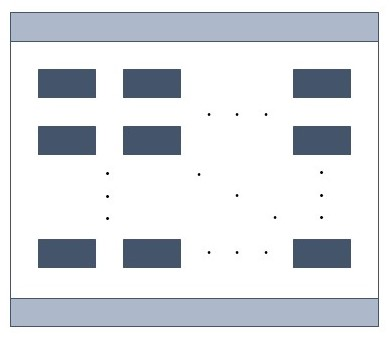
\includegraphics[scale=0.5]{figures/Warehouse_gen.jpg}
    \caption{倉庫の構成}
    \label{fig:Warehouse_gen}
\end{figure}

すべてのロボットにおいて,商品を積み込むときを除いて,いかなるときも棚に侵入できない.そして,棚に侵入するときは必ず上から入り下から出ていく.また,ロボットは前もしくは,右か左に進む動きしかできず,後ろ向きには進めないものとする.

ロボットは上の待機場所でタスクを割り当てられるのを待ち,割り当てられたら目的の品があるところまで行き,商品を積み,下の搬出場所までいく.ここでのタスクを割り当てられるというのは,スタート地点,ゴール地点,商品の場所の3つを与えられることである.スタート地点は待機場所の一段下の状態を,ゴール地点は搬出場所の一段上の状態を指す.商品の場所は棚のうちの一つを指す.

そして人間は、通常下で作業しており,トラブルが発生したときや,人間の協力が必要になったとき,ロボットも通る通路を使って目的の場所まで行く.また,人間はスーパーバイザの制御対象ではない.つまり,人間を制御できない対象として制御システム扱う必要がある.

また,倉庫内で複数台のロボットを制御するとき,以下の点において,注意する必要がある.
\begin{itemize}
    \item 安全性:ロボット同士や人間とロボットの接触(衝突)を防ぐ
    \item デッドロック状態の回避:図のように,お互いのロボットが道を塞いでしまい,動けなくなる状態になることを回避する
    \item 効率性:すべてのロボットが荷物を届け終えるまでの時間が最短になるようにする
\end{itemize}
安全性については,ロボットだけの制御が場合,2台のロボットが同じ状態に存在することを禁止する条件を,すべてのロボットの組み合わせで定めて制御要求として与える.スーパーバイザによってロボットの衝突を回避することが可能になる.
しかし,この制御に人間が加わるとなると,より高度な安全性を考える必要がある.

デッドロック状態は図\ref{fig:Dead_Lock}のようにお互い進めなくなる状況である.これはノンブロッキングであることをスーパーバイザに要求することで解決される.
%あとは効率性の説明

\begin{figure}[h]
    \centering
    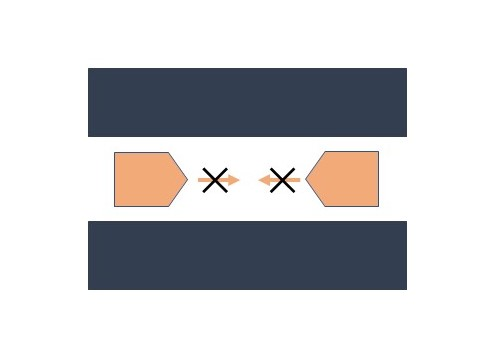
\includegraphics[scale=0.5]{figures/Dead_Lock.jpg}
    \caption{デッドロック状態}
    \label{fig:Dead_Lock}
\end{figure}


\section{ロボットのモデル化}\label{sec:design_robot}

倉庫内のロボットはすべてオートマトンで設計する.第2章で紹介したオートマトンのように5つの要素で構成する$n(>1)$台のロボットを考えるとき,ロボットのオートマトンを以下の$G_i(i=1,2,\ldots,n)$で定義する.
\begin{equation}
    G_i=(Q_i,\Sigma_i,\delta_i,q_{0,i},Q_{m,i})
\end{equation}
ここで$Q_i$は$i$台目のロボットの最短経路上の全状態の集合,$\Sigma_i$は$i$台目のロボットの動作の集合,$\delta_i$は状態遷移関数,$q_{0,i}$は待機場所の状態,$Q_{m,i}$は搬出場所の状態で構成されている.ロボットの動作は表\ref{tb:event_numbers}にあるように設定する.TCTでは奇数の事象が可制御事象,偶数の事象が不可制御事象として処理される.ロボットの動作はすべて可制御事象なので奇数で与える.ここでは北,東,南,西に進むと記載しているが,図で示す場合,それぞれ上,右,下,左で表す.

\begin{table}[htb]
    \centering
    \begin{tabular}{|c|c|} \hline
        事象 & 番号 \\ \hline
        北へ進む & $i\times10+1$ \\
        東へ進む & $i\times10+3$ \\
        南へ進む & $i\times10+5$ \\
        西へ進む & $i\times10+7$ \\ \hline
    \end{tabular}
    \caption{$i$台目のロボットの事象に振られる番号}
    \label{tb:event_numbers}
\end{table}

\section{人間のモデル化}

倉庫内の人間も,ロボットと同様にオートマトンで定義する.人間が$m$人倉庫内に立ち入るとする.ある人間$H_j(j=1,2,\cdots ,m)$の普段の作業場所である一番下の位置(搬出場所)を初期状態$q_{0,H_j}$,戻るべき目的地を$Q_{m,H_j}$,最短経路上の全状態の集合を$\Sigma_{H_j}$状態遷移関数を$\delta_{H_j}$とおいて,人間のオートマトンを以下で表す.

\begin{equation}
H_j=(Q_{H_j},\Sigma_{H_j},\delta_{H_j},q_{0,H_j},Q_{m,H_j})
\end{equation}

人間とロボットが存在する倉庫では,人間の安全面を絶対に確保することが求められ,最優先に考える必要があり,第4章で解説する.


\section{スーパーバイザの設計}\label{sec:design_sup}
スーパーバイザを計算する手順について解説する.

本研究ではTCTという離散事象システムの計算に特化したソフトウェアを使用し,計算を行う.

$N$個の要素(エージェント)と$K$個の制御要求が与えられたとする.

$n$台のロボットの初期状態,受理状態,状態遷移をもとに,それぞれのオートマトン$G_1,G_2,\cdots,G_n$を作成する.また,人間のオートマトン$H_1, H_2, \cdots, H_m$も作成する.$n$と$m$について,$n+m=N$と書くことができる.

%そして,2つのオートマトンの状態のペアを与えて,同時刻に2つのオートマトンそれぞれが与えられた状態のペア存在することを禁止する関数mutexを使用して,制御要求のオートマトン$E_1,E_2,\cdots,E_K$を作成する.
2つのオートマトンに対して,2つの状態で構成される状態のペアを与えられると,オートマトンそれぞれが状態のペアの状態に同時に存在しないようにする関数mutexという関数がある.この関数で出力されるオートマトンを,制御要求のオートマトン$E_1,E_2,\cdots,E_K$とする.

次に,$G_1,\cdots,G_n,H_1,\cdots,H_m$のすべてのオートマトンを同期合成させ,制御対象であるPLANTを出力する.このとき,受理状態のみ存在し,PLANTのすべての事象で自己ループする遷移が定義されるオートマトンALLを作成する.

$E_1$から$E_K$までのすべての制御要求とPLANTの全事象を含んだALLを同期合成させ,制御要求SPECを生成する.

Supconと呼ばれる関数にPLANTとSPECを入力し,制御要求を満たすスーパーバイザを得る.

